\section{Exact solutions for simple cases}\label{sec:exactSolutions}

In \ac{PHS} form, the Hubbard Hamiltonian may then be written as a sum of kinetic and chemical, and potential energy terms 
$
\mathcal{H} = \mathcal{H}_K + \mathcal{H}_V ,
$
defined as

\begin{equation}\label{eq:def_energies}
\mathcal{H}_K = -t \sum_{\left\langle i, j \right \rangle, \sigma} \bigg( c_{i,\sigma} c_{j,\sigma}^\dagger + c_{j,\sigma}^\dagger c_{i,\sigma} \bigg) -\mu \sum_i \bigg( n_{i,\uparrow} + n_{i,\downarrow} \bigg) , \,\,\,
\mathcal{H}_V = U \sum_{i} \bigg( n_{i,\uparrow} - \frac{1}{2} \bigg) \bigg( n_{i,\downarrow} - \frac{1}{2} \bigg) ,
\end{equation}
where $i$ and $j$ label sites on the lattice; $c_{i,\sigma}^{(\dagger)}$ is an operator that annihilates (creates) an electron with spin $\sigma$ on site $i$; $n_{i,\sigma}$ is the number operator counting the number of electrons of spin $\sigma$ on site $i$ (either 0 or 1); $t$ is the hopping parameter related to the kinetic energy of the electrons: it is determined by the overlap of the atomic wave functions on neighboring sites $\left\langle i, j \right\rangle$; $U$ is the on-site Coulomb repulsion between electrons: whenever a site $i$ has two electrons, there is a local repulsion between them corresponding to an energy cost $U n_{i \uparrow} n_{i \downarrow}$ (up to an additive constant); $\mu$ is the chemical potential controlling the electron number (or density).

A given physical observable of interest $\mathcal{O}$, such as the spin-spin correlation, or the magnetic susceptibility may be computed formally by

\begin{equation}
\left\langle \mathcal{O} \right\rangle = \text{Tr} ( \mathcal{O} \mathcal{P} )
\end{equation}
where

\begin{equation}\label{eq:projection}
\mathcal{P} \equiv \frac{1}{Z} e^{-\beta \mathcal{H} } , \text{ with } Z = \text{Tr} ( e^{-\beta \mathcal{H} } )
\end{equation}

The trace is taken over the Hilbert space corresponding to all possible configurations of the lattice occupation.
Defining an orthonormal basis of this Hilbert space $\{ | \psi_\alpha \rangle | \alpha = 1, ... D \} $, where $D$ is the dimension of the Hilbert space, the partition function reads

\begin{equation}\label{eq:z_asEigen}
\Tr ( e^{-\beta \mathcal{H} } )= \sum_\alpha \left\langle \psi_\alpha | e^{-\beta \mathcal{H} } | \psi_\alpha \right\rangle
\end{equation}

There are four possible states at each site in the Hubbard model: $\left| \,\, \right\rangle$, $\left|\uparrow \right\rangle$, $\left|\downarrow\right \rangle$, $\left|\uparrow \downarrow \right\rangle $, corresponding, respectively, to no electron, a spin up or spin down electron, and two electrons of opposite spin occupying the site.
The potential energy operator acts as follows

\begin{equation}
U (n_{i\uparrow} - \frac{1}{2} ) ( n_{i\downarrow} - \frac{1}{2} ) 
\begin{cases}
\left| \,\, \right\rangle = \frac{U}{4} \left| \,\, \right\rangle \\
\left|\uparrow \right\rangle = -\frac{U}{4} \left|\uparrow \right\rangle \\
\left|\downarrow\right \rangle = -\frac{U}{4} \left|\downarrow\right \rangle \\
\left|\uparrow \downarrow \right\rangle = \frac{U}{4} \left|\uparrow \downarrow \right\rangle \\
\end{cases}
\end{equation}

Singly occupied states ($\left|\uparrow \right\rangle$, $\left|\downarrow\right \rangle$) have lower energy and are thus more likely to occur.
They correspond to nonzero magnetization $m = n_{\uparrow} - n_{\downarrow}$, which is favored by the Hubbard interaction $U$.
A relevant question is whether or not the spins order in space when $t \neq 0$ and to what extent.

Let us now establish our notations for second quantized operators to introduce a different representation of electronic states on the lattice.
The fermionic annihilation and creation operators anticommute:
$\{ c_{j\sigma} , c_{l \sigma'}^\dagger \} = \delta_{jl} \delta_{\sigma\sigma'}$.
The $c$-operator algebra is further defined by the vanishing of all other anticommutators:$
\{ c_{j\sigma}^{(\dagger)} , c_{l \sigma'}^{(\dagger)} \} = 0$.
Note that taking $l = j$ and $\sigma = \sigma'$ in this equation for the $c^\dagger$-operators, we recover Pauli's exclusion principle since $(c_{j\sigma}^\dagger)^2 = 0$.
If we omit the site $i$ and spin $\sigma$ indices, a convenient way of specifying states on the lattice is

\begin{equation}
\left| 0 \right\rangle : \text{unoccupied state - no electron} \,\,\,\, \left| 1 \right\rangle : \text{occupied state - one electron}
\end{equation}
so that a generic state may be written as a product of the states above $\otimes_{i=1}^{N} \otimes_{\sigma = \pm 1/2} \left| n \right\rangle_{i, \sigma}$ at each site for each spin state, where $n= 0, 1$.
For example, one such state is

\begin{equation}
\left| 0 \right\rangle_{1, \uparrow} \left| 1 \right\rangle_{1, \downarrow} \left| 1 \right\rangle_{2, \uparrow} \left| 1 \right\rangle_{2, \downarrow} \left| 0 \right\rangle_{3, \uparrow} \left| 0 \right\rangle_{3, \downarrow} ... \left| 1 \right\rangle_{N, \uparrow} \left| 0 \right\rangle_{N, \downarrow}  ,
\end{equation}
where $N$ is the number of sites on the lattice. Site $1$ has a single spin-down electron, while site $2$ is doubly occupied, site $3$ is unoccupied, and so on, until we reach site $N$, which has a single spin-up electron.
The creation and annihilation operators act as follows

\begin{equation}
c \left| 0 \right\rangle = 0 \quad c^\dagger \left| 0 \right\rangle = \left| 1 \right\rangle \quad c \left| 1 \right\rangle = \left| 0 \right\rangle \quad c^\dagger \left| 1 \right\rangle = 0
\end{equation}

Thus, the eigenstates of the number operator are $\left| 0 \right\rangle, \left| 1 \right\rangle$: $
n \left| 0 \right\rangle = 0 , \, n \left| 1 \right\rangle = \left| 1 \right\rangle
$.
Moreover, the operator $c_i^\dagger c_{i+1}^\dagger$, corresponding to the hopping from site $i+1$ to $i$, i.e. to the kinetic energy of the electrons on neighboring sites, annihilates the particle at $i+1$ and creates it back at $i$, i.e. the electron hops from $i+1$ to $i$.
Ignoring spin:

\begin{equation}
c_i^\dagger c_{i+1}^\dagger \begin{cases}
\left|0 0 \right\rangle = 0 \\
\left|1 0 \right\rangle =  0 \\
\left|0 1 \right\rangle =  \left| 1 0 \right\rangle \\
\left|1 1 \right\rangle =  c_i^\dagger \left| 1 0  \right\rangle = 0 \\
\end{cases}
\end{equation}

\subsection{The purely atomic ( $\frac{U}{t} \rightarrow \infty$ ), single site limit}
\label{subsec:atomic}

When $t = 0$, the site index may be omitted since the Hamiltonian is a sum of operators solely at site $i$.
Hence, we have $[ \mathcal{H}, n_{i,\sigma} ] = 0 \,\, \forall i = 1, 2,..., N $, and the eigenstates of $\mathcal{H}$ are also eigenstates of all number operators at the different sites in the lattice.
Thus, in the single site limit, we obtain

\begin{equation}
\mathcal{H} = U \bigg(n_\uparrow - \frac{1}{2} \bigg) \bigg(n_\downarrow - \frac{1}{2} \bigg) - \mu \bigg( n_\uparrow + n_\downarrow \bigg)
\end{equation}
which acts as follows (using the eigenstates of $n_\sigma$)

\begin{equation}
\mathcal{H} \begin{cases}
\left| \,\, \right\rangle = \frac{U}{4} \left| \,\, \right\rangle \\
\left| \uparrow \right\rangle = \bigg( \frac{U}{4} - (\mu + \frac{U}{2} ) \bigg) \left| \uparrow \right\rangle \\
\left| \downarrow \right\rangle = \bigg( \frac{U}{4} - (\mu + \frac{U}{2} ) \bigg) \left| \downarrow \right\rangle \\
\left| \uparrow \downarrow \right\rangle = \bigg( \frac{U}{4} - 2 \mu \bigg) \left| \uparrow \downarrow \right\rangle
\end{cases}
\end{equation}

Thus, the Hamiltonian is diagonal in the basis $\{\left| \psi_\alpha \right\rangle \} = \left| \,\, \right\rangle, \left|\uparrow \right\rangle, \left|\downarrow\right \rangle, \left|\uparrow \downarrow \right\rangle $:

\begin{equation}
\mathcal{H} \leadsto \bm H = \text{diag}\bigg(\frac{U}{4}, \frac{U}{4} - (\mu + \frac{U}{2} ), \frac{U}{4} - (\mu + \frac{U}{2} ), \frac{U}{4} - 2 \mu \bigg) ,
\end{equation}
which means that $e^{-\beta \mathcal{H} }$ is also diagonal:

\begin{equation}
e^{-\beta \mathcal{H} } \leadsto e^{-\beta U / 4}  \text{diag}\bigg(1,  e^{\beta(\mu + \frac{U}{2})}, e^{\beta(\mu + \frac{U}{2})},  e^{2\beta \mu} \bigg)
\end{equation}
and this is one of the rare situations in which it is possible to explicitly write down a closed form for the partition function.

\begin{equation}\label{eq:singleSitePartition}
Z = \text{Tr} [ e^{-\beta\mathcal{H} } ] = \sum_\alpha \left\langle \psi_\alpha \left|e^{-\beta \mathcal{H} } \right| \psi_\alpha \right\rangle = e^{-\beta U / 4} \bigg(1 + 2 e^{\beta(\mu + \frac{U}{2})} + e^{2 \beta \mu} \bigg)
\end{equation}

Moreover, some of the observables that were mentioned before are explicitly computable.
This is because due to the diagonal form of $\mathcal{H}$, the expressions defining these observables greatly simplify.

\begin{equation}
\begin{split}
\mathcal{H} e^{-\beta\mathcal{H} } &\leadsto e^{-\beta U / 4}  \text{diag}\bigg(\frac{U}{4}, (-\mu - \frac{U}{4})  e^{\beta(\mu + \frac{U}{2})} (-\mu - \frac{U}{4}) e^{\beta(\mu + \frac{U}{2})}, (\frac{U}{4} - 2\mu ) e^{2\beta \mu} \bigg) \\
n_{\uparrow} e^{-\beta\mathcal{H} } &\leadsto e^{-\beta U / 4}  \text{diag}\bigg(0, e^{\beta(\mu + \frac{U}{2})}, 0,  e^{2\beta \mu} \bigg) \\
n_{\downarrow} e^{-\beta\mathcal{H} } &\leadsto e^{-\beta U / 4}  \text{diag}\bigg(0, 0, e^{\beta(\mu + \frac{U}{2})},   e^{2\beta \mu} \bigg) \\
n_{\uparrow} n_{\downarrow} e^{-\beta\mathcal{H} } &\leadsto e^{-\beta U / 4}  \text{diag}\bigg(0, 0, 0,   e^{2\beta \mu} \bigg) \\
\end{split}
\end{equation}

From these we can compute some traces which we shall find useful to obtain averages of various observables.

\begin{equation}
\begin{split}
&\Tr \bigg[ \mathcal{H} e^{-\beta\mathcal{H} } \bigg] = e^{-\beta U / 4} \bigg(\frac{U}{4} + 2 (-\mu - \frac{U}{4})  e^{\beta(\mu + \frac{U}{2})} + (\frac{U}{4} - 2\mu ) e^{2\beta \mu} \bigg) \\
&\Tr \bigg[ (n_\uparrow + n_\downarrow ) e^{-\beta\mathcal{H} } \bigg] = e^{-\beta U / 4} \bigg(2 (-\mu - \frac{U}{4})  e^{\beta(\mu + \frac{U}{2})} + (\frac{U}{4} - 2\mu ) e^{2\beta \mu} \bigg) \\
&\Tr \bigg[ n_\uparrow n_\downarrow \bigg] = e^{-\beta U/4} e^{2\beta\mu}
\end{split}
\end{equation}

The bottom line is that we are able to obtain \emph{exact} expressions for

\begin{enumerate}
\item the one-site density $\rho = \left\langle n_\uparrow \right\rangle + \left\langle n_\downarrow \right\rangle$, measuring the average occupation of each site.
\begin{equation}
\rho = \frac{\text{Tr} \big[ (n_\uparrow + n_\downarrow ) e^{-\beta\mathcal{H}} \big]}{Z} = \frac{2 e^{\beta(\frac{U}{2} + \mu)} + 2 e^{2\beta\mu}}{1 + 2 e^{\beta(\mu + \frac{U}{2})} + e^{2 \beta \mu}}
\end{equation}

Note that when there is no chemical potential $\mu = 0$, we have $\rho = 1$ for any $U$, or $\beta$.
This corresponds to half filling: the density of electrons is half its maximum possible value.

In Fig. (\ref{fig:rhoVsMu}), we plot $\rho(\mu)$ for varying temperature, and fixed on-site interaction.
It allows us to get some insight into the Mott insulating gap.
At $T = 0.25$, the curve owes its step-like shape to the small thermal fluctuations.
As $T$ increases, the curve starts losing this tendency, and by $T = 2.0$, it is no longer possible to identify it.
This is a consequence of the now larger thermal fluctuations that are present at higher temperature.
We denote the flat region between $\mu = - U / 2 $ and $\mu =  U / 2 $  \say{Mott Plateau}.
As the chemical potential is increased, the density remains small until a threshold is exceeded at $\mu = - \frac{U}{2}$. 
Then, it rises very rapidly to $\rho = 1$ (half filling), and again stays almost constant.
It is not until $\mu$ jumps by $U$ that we fill the site ($\rho = 2$).
This Mott insulating gap appears because the presence of a fermion in the site blocks the addition of a second one due to the on-site interaction.
One needs a sufficiently large chemical potential to overcome this effect.
As we shall see, this feature of the model remains present as the number of sites increases.
Note that in the Mott gap, the compressibility vanishes: $\kappa = \frac{\partial \rho}{\partial \mu} = 0$, leading to the appearance of the Mott Plateau.
Just as thermal fluctuations can destroy the sharp jumps corresponding to the gap, so can quantum fluctuations.
The hopping term in the Hamiltonian introduces such fluctuations, leading to an effect similar to that of Fig.  (\ref{fig:rhoVsMu}).
\begin{figure}[H]
	\centering
\hspace{12mm}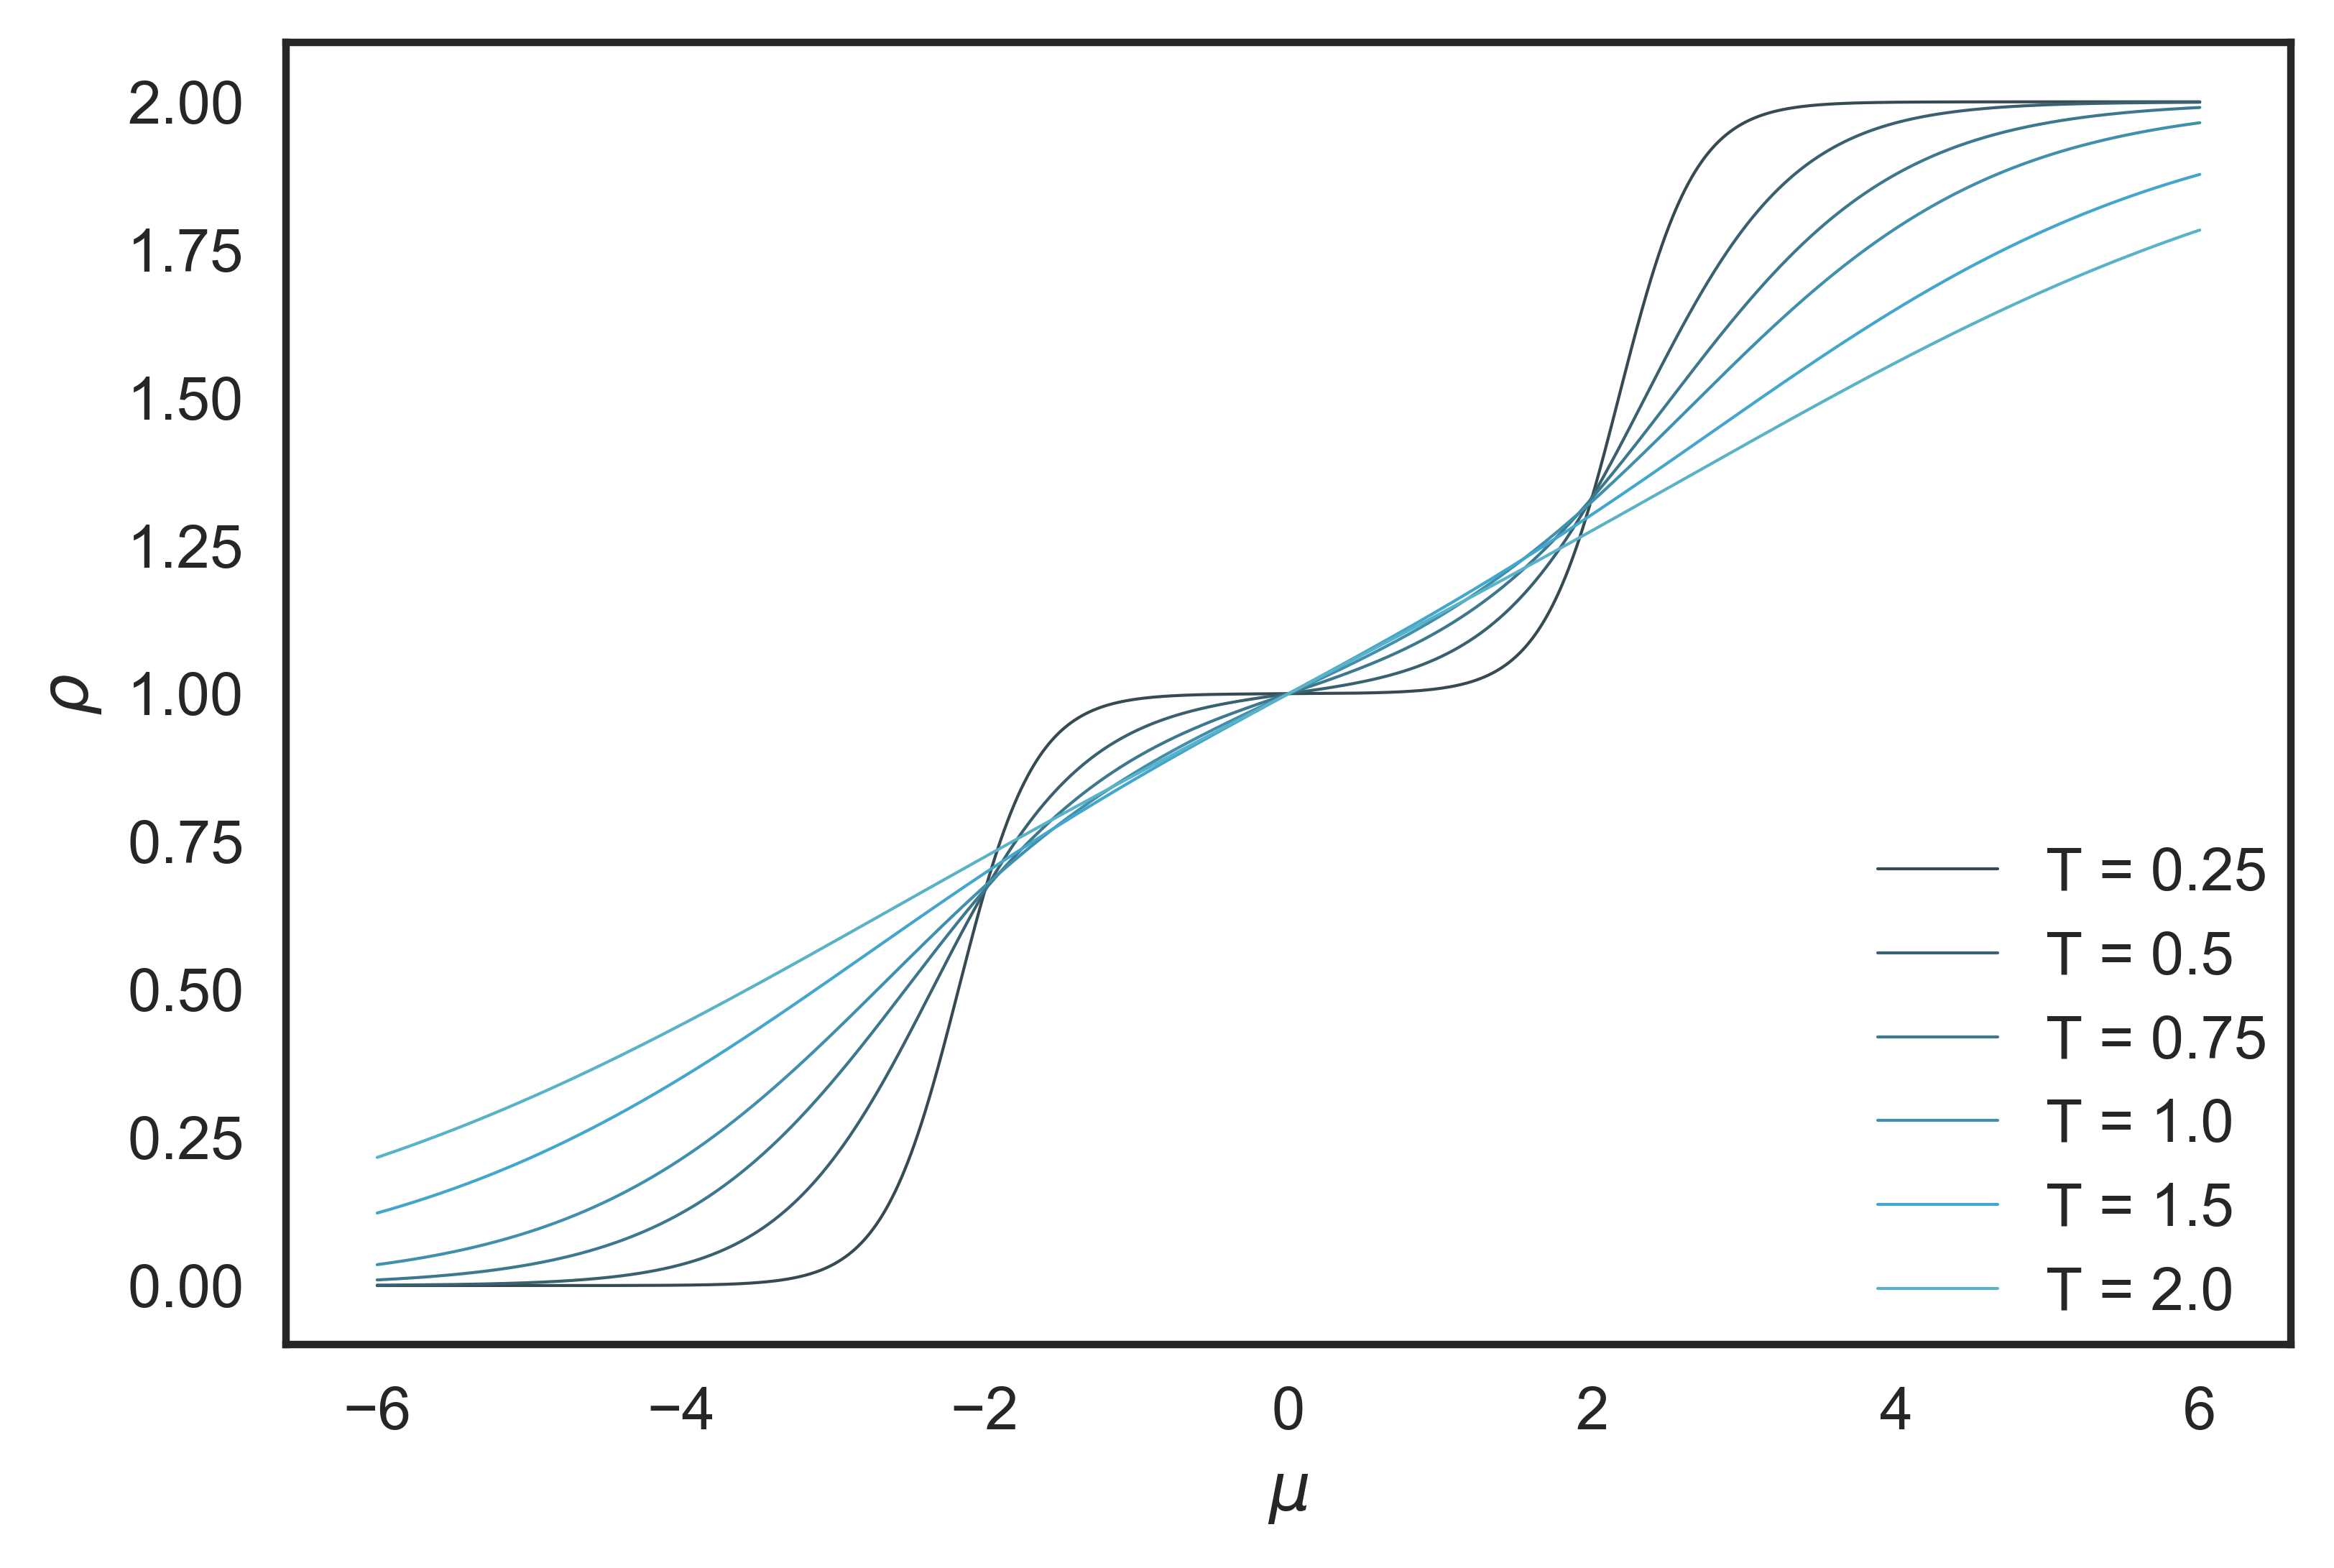
\includegraphics[width=0.7\linewidth]{Hubbard/rhoVsMu.png}
	\caption[Electron density in the purely atomic limit of the Hubbard model]{Electron density $\rho$ for varying chemical potential $\mu$ and temperature $T = \beta^{-1}$, but fixed $U = 4$. As the temperature decreases, a \say{Mott plateau} sets in. The Mott insulating gap already seen here is an important feature of the Hubbard model.}
	\label{fig:rhoVsMu}
\end{figure}

\item the one-site energy $E = \left\langle \mathcal{H} \right\rangle$.
\begin{equation}
\begin{split}
E &= \frac{\text{Tr}\bigg( \mathcal{H}e^{-\beta\mathcal{H} } \bigg)}{Z} = \frac{ \frac{U}{4} + 2 ( -\mu - \frac{U}{4} ) e^{\beta(\frac{U}{2} + \mu )} + (\frac{U}{4} - 2\mu ) e^{2\beta\mu}}{1 + 2 e^{\beta (\frac{U}{2} + \mu )} + e^{2\beta\mu} } \\
&= \frac{ \frac{U}{4} ( 1 + 2 e^{\beta (\frac{U}{2} + \mu )} + e^{2\beta\mu} )}{1 + 2 e^{\beta (\frac{U}{2} + \mu )} + e^{2\beta\mu} } + \frac{2(-\mu - \frac{U}{4}) e^{\beta(\frac{U}{2} + \mu)} - 2\mu e^{2\beta\mu} - 2\frac{U}{4} e^{\beta (\frac{U}{2} + \mu)} }{1 + 2 e^{\beta (\frac{U}{2} + \mu )} + e^{2\beta\mu}} \\
&= \frac{U}{4} - \frac{ (2\mu - U) e^{\beta(\frac{U}{2} + \mu) } + 2\mu e^{2\beta\mu} }{1 + 2 e^{\beta (\frac{U}{2} + \mu )} + e^{2\beta\mu} }
\end{split}
\end{equation}
which at half filling becomes

\begin{equation}
E = \frac{U}{4} - \frac{U}{2 ( 1 + e^{-\beta U /2} )}
\end{equation}

\item the double occupancy $\left\langle n_\uparrow n_\downarrow \right\rangle$.

\begin{equation}
\left\langle n_\uparrow n_\downarrow \right\rangle = \frac{\text{Tr} \big[ n_\uparrow n_\downarrow \big]}{Z} = \frac{e^{2\beta\mu}}{1 + 2 e^{\beta (\frac{U}{2} + \mu )} + e^{2\beta\mu}}
\end{equation}
which, at half filling, simplifies to

\begin{equation}
\left\langle n_\uparrow n_\downarrow \right\rangle = \frac{1}{2 ( 1 + e^{\beta U/2} )}
\end{equation}

Note that as either $U$ or $\beta$ increase the double occupancy tends to zero.
\end{enumerate}

As was motivated in the previous chapter, we are interested in studying magnetism in correlated systems.
For the Hubbard model, the relevant quantity is the local moment

\begin{equation}
\left\langle m^2 \right\rangle = \left\langle ( n_\uparrow - n_\downarrow )^2 \right\rangle = \left\langle n_\uparrow - n_\downarrow \right\rangle - 2  \left\langle n_\uparrow n_\downarrow \right\rangle = \rho - 2  \left\langle n_\uparrow n_\downarrow \right\rangle
\end{equation}

In Figs. (\ref{fig:mSqVsU}, \ref{fig:mSqVsT}), we show how $\left\langle m^2 \right\rangle$ varies as a function of $U$ for different temperatures, and how $\left\langle m^2 \right\rangle$ varies with $T$, for different values of the chemical potential, respectively.
At low temperature or for large on-site interaction, local moments tend to develop, which leads to magnetic ordering: $\left\langle m^2 \right\rangle \rightarrow 1$ (in the half-filled case).
Since the double occupancy is zero in this case, if we do not consider thermal fluctuations, the magnetization corresponds to the spin of the electron occupying the site.

\begin{figure}[H]
	\centering
\hspace{12mm}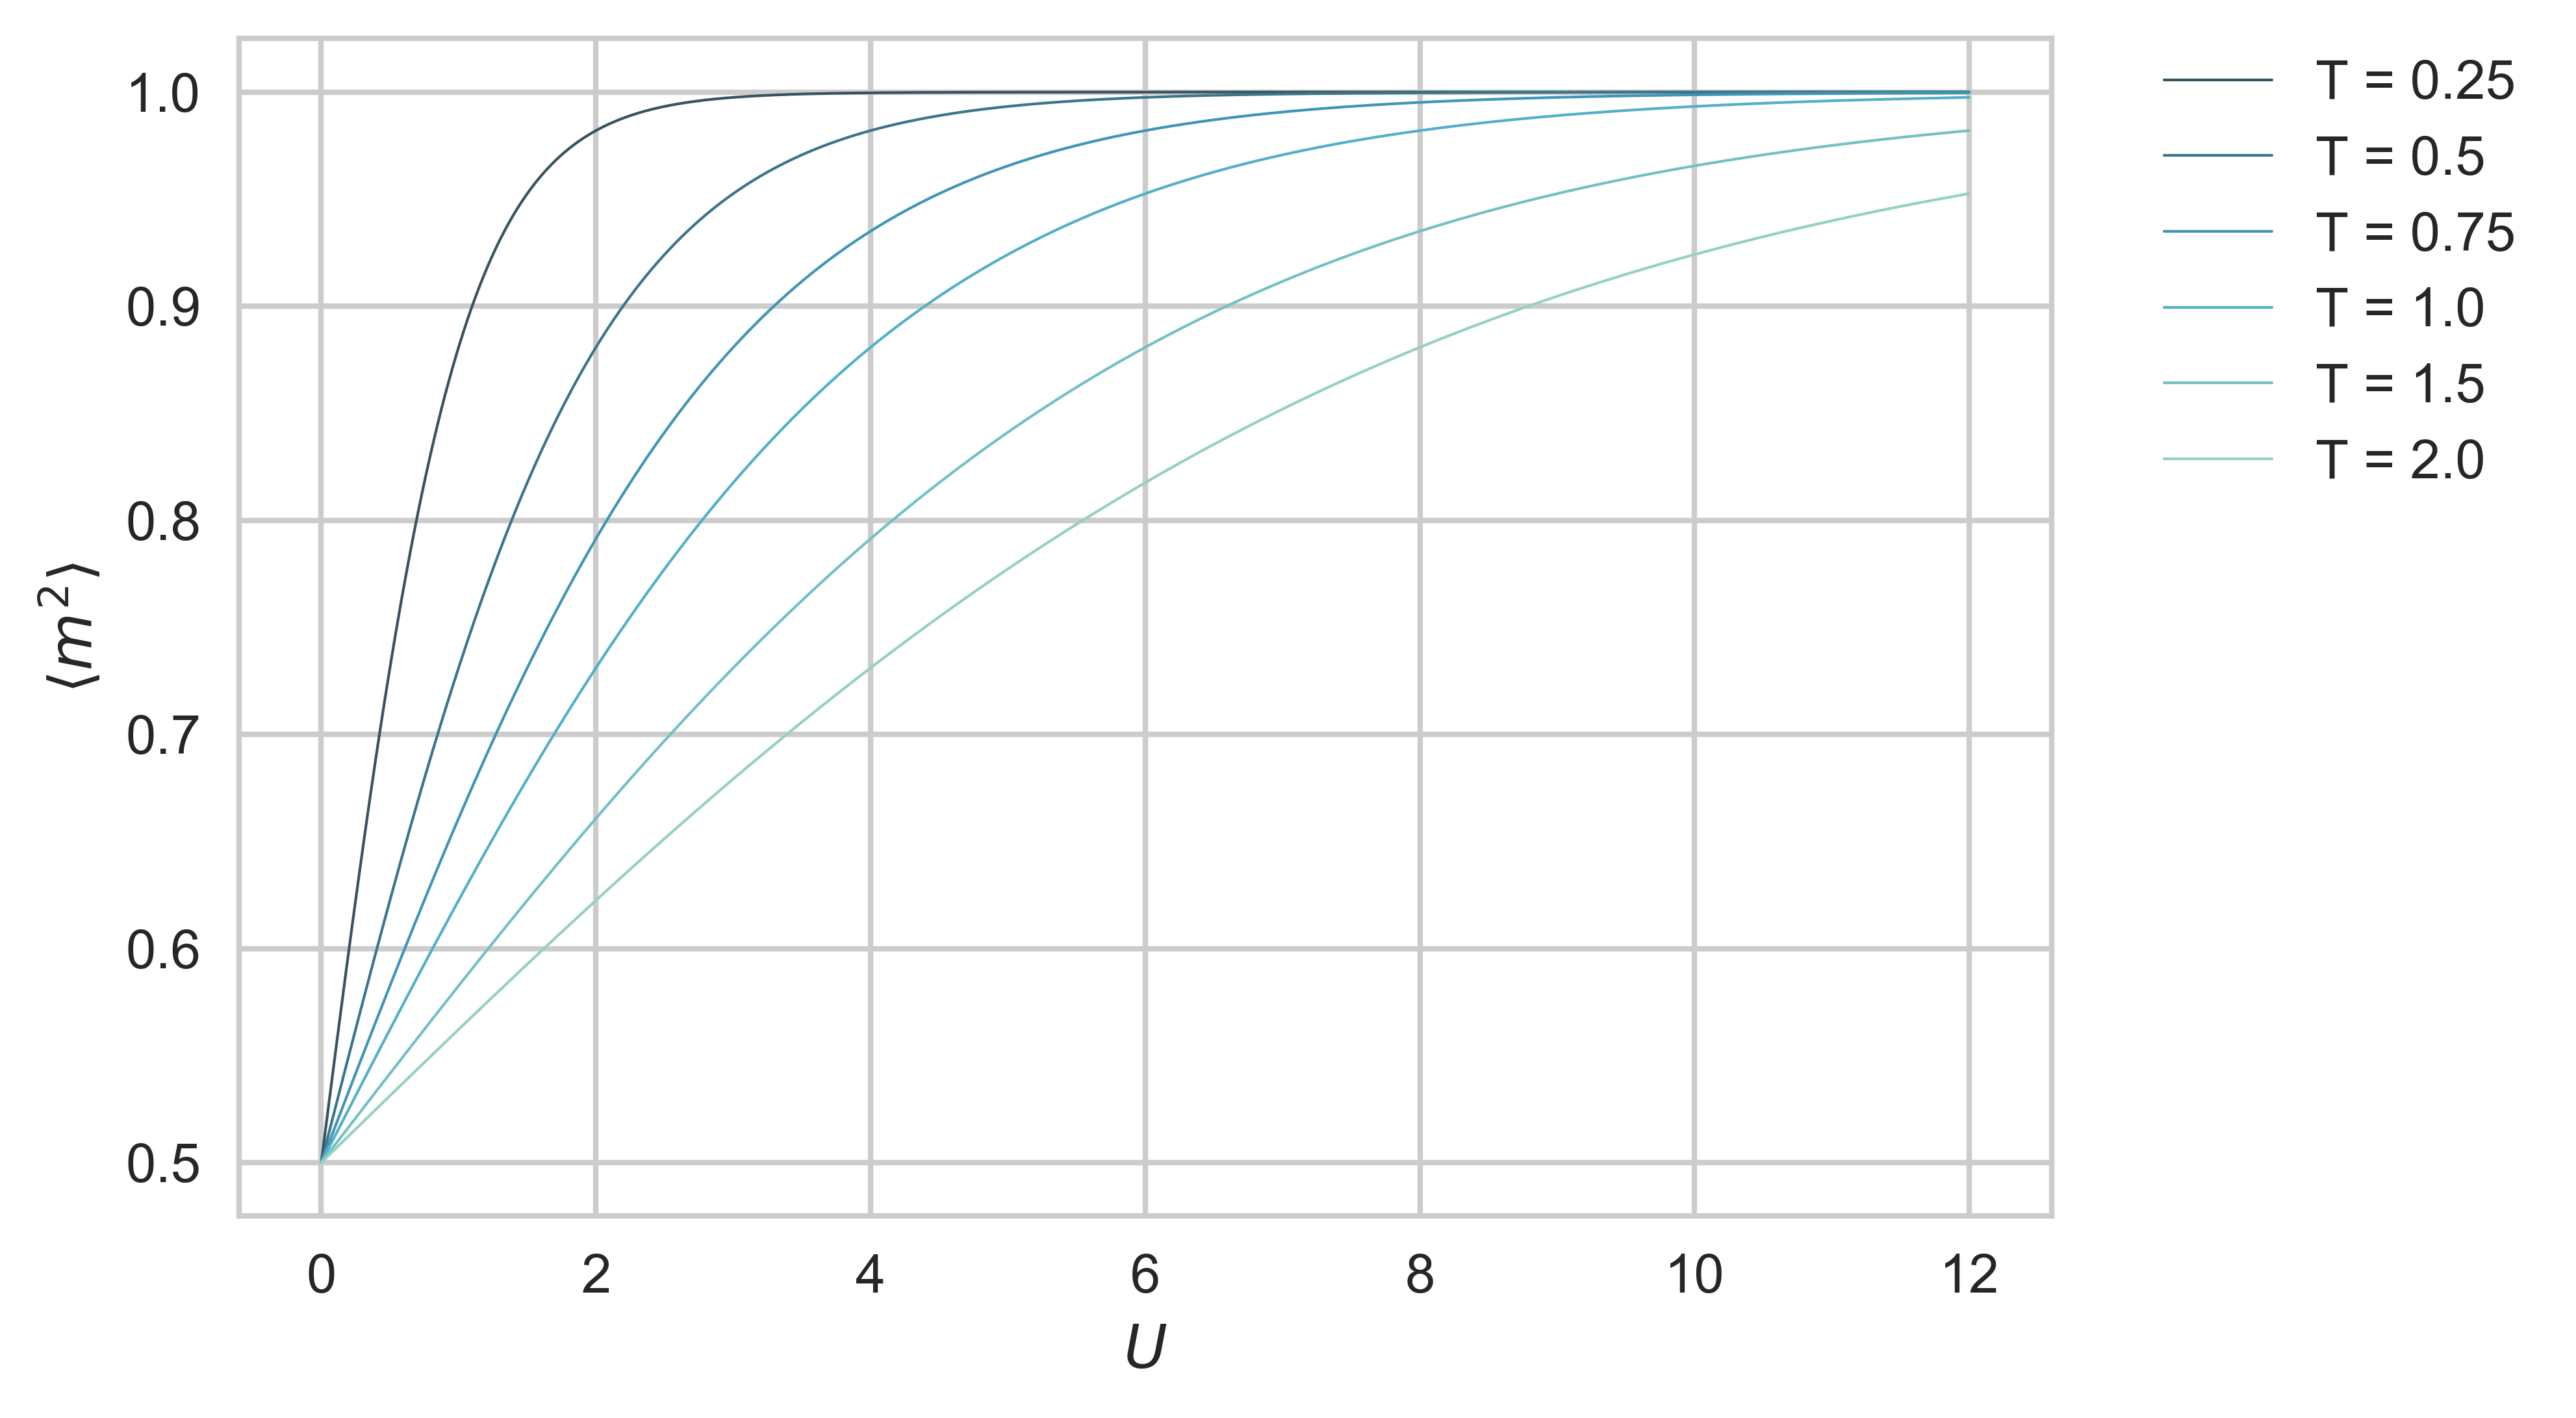
\includegraphics[width=0.7\linewidth]{Hubbard/mSqVsU.png}
	\caption[Magnetization as a function of the on-site interaction $\left\langle m^2 \right\rangle (U)$ in the single site Hubbard model for varying temperature $T$.]{Magnetization as a function of the on-site interaction $\left\langle m^2 \right\rangle (U)$ in the single site Hubbard model for varying temperature $T$.
	Local moments are favored by the on-site interaction, and are more likely to develop at lower temperatures, when thermal fluctuations are smaller. Here we consider half filling: $\mu = 0$.}
	\label{fig:mSqVsU}
\end{figure}

In Fig. (\ref{fig:mSqVsU}), we see thermal fluctuations destroying magnetic ordering.
As what happens for the Mott plateau, quantum fluctuations (i.e. introducing a hopping term in the Hamiltonian) change the behavior of the magnetization, and perfect moments ($\left\langle m^2 \right\rangle =1$) do not form anymore at zero temperature for finite on-site interaction.

\begin{figure}[H]
	\centering
\hspace{12mm}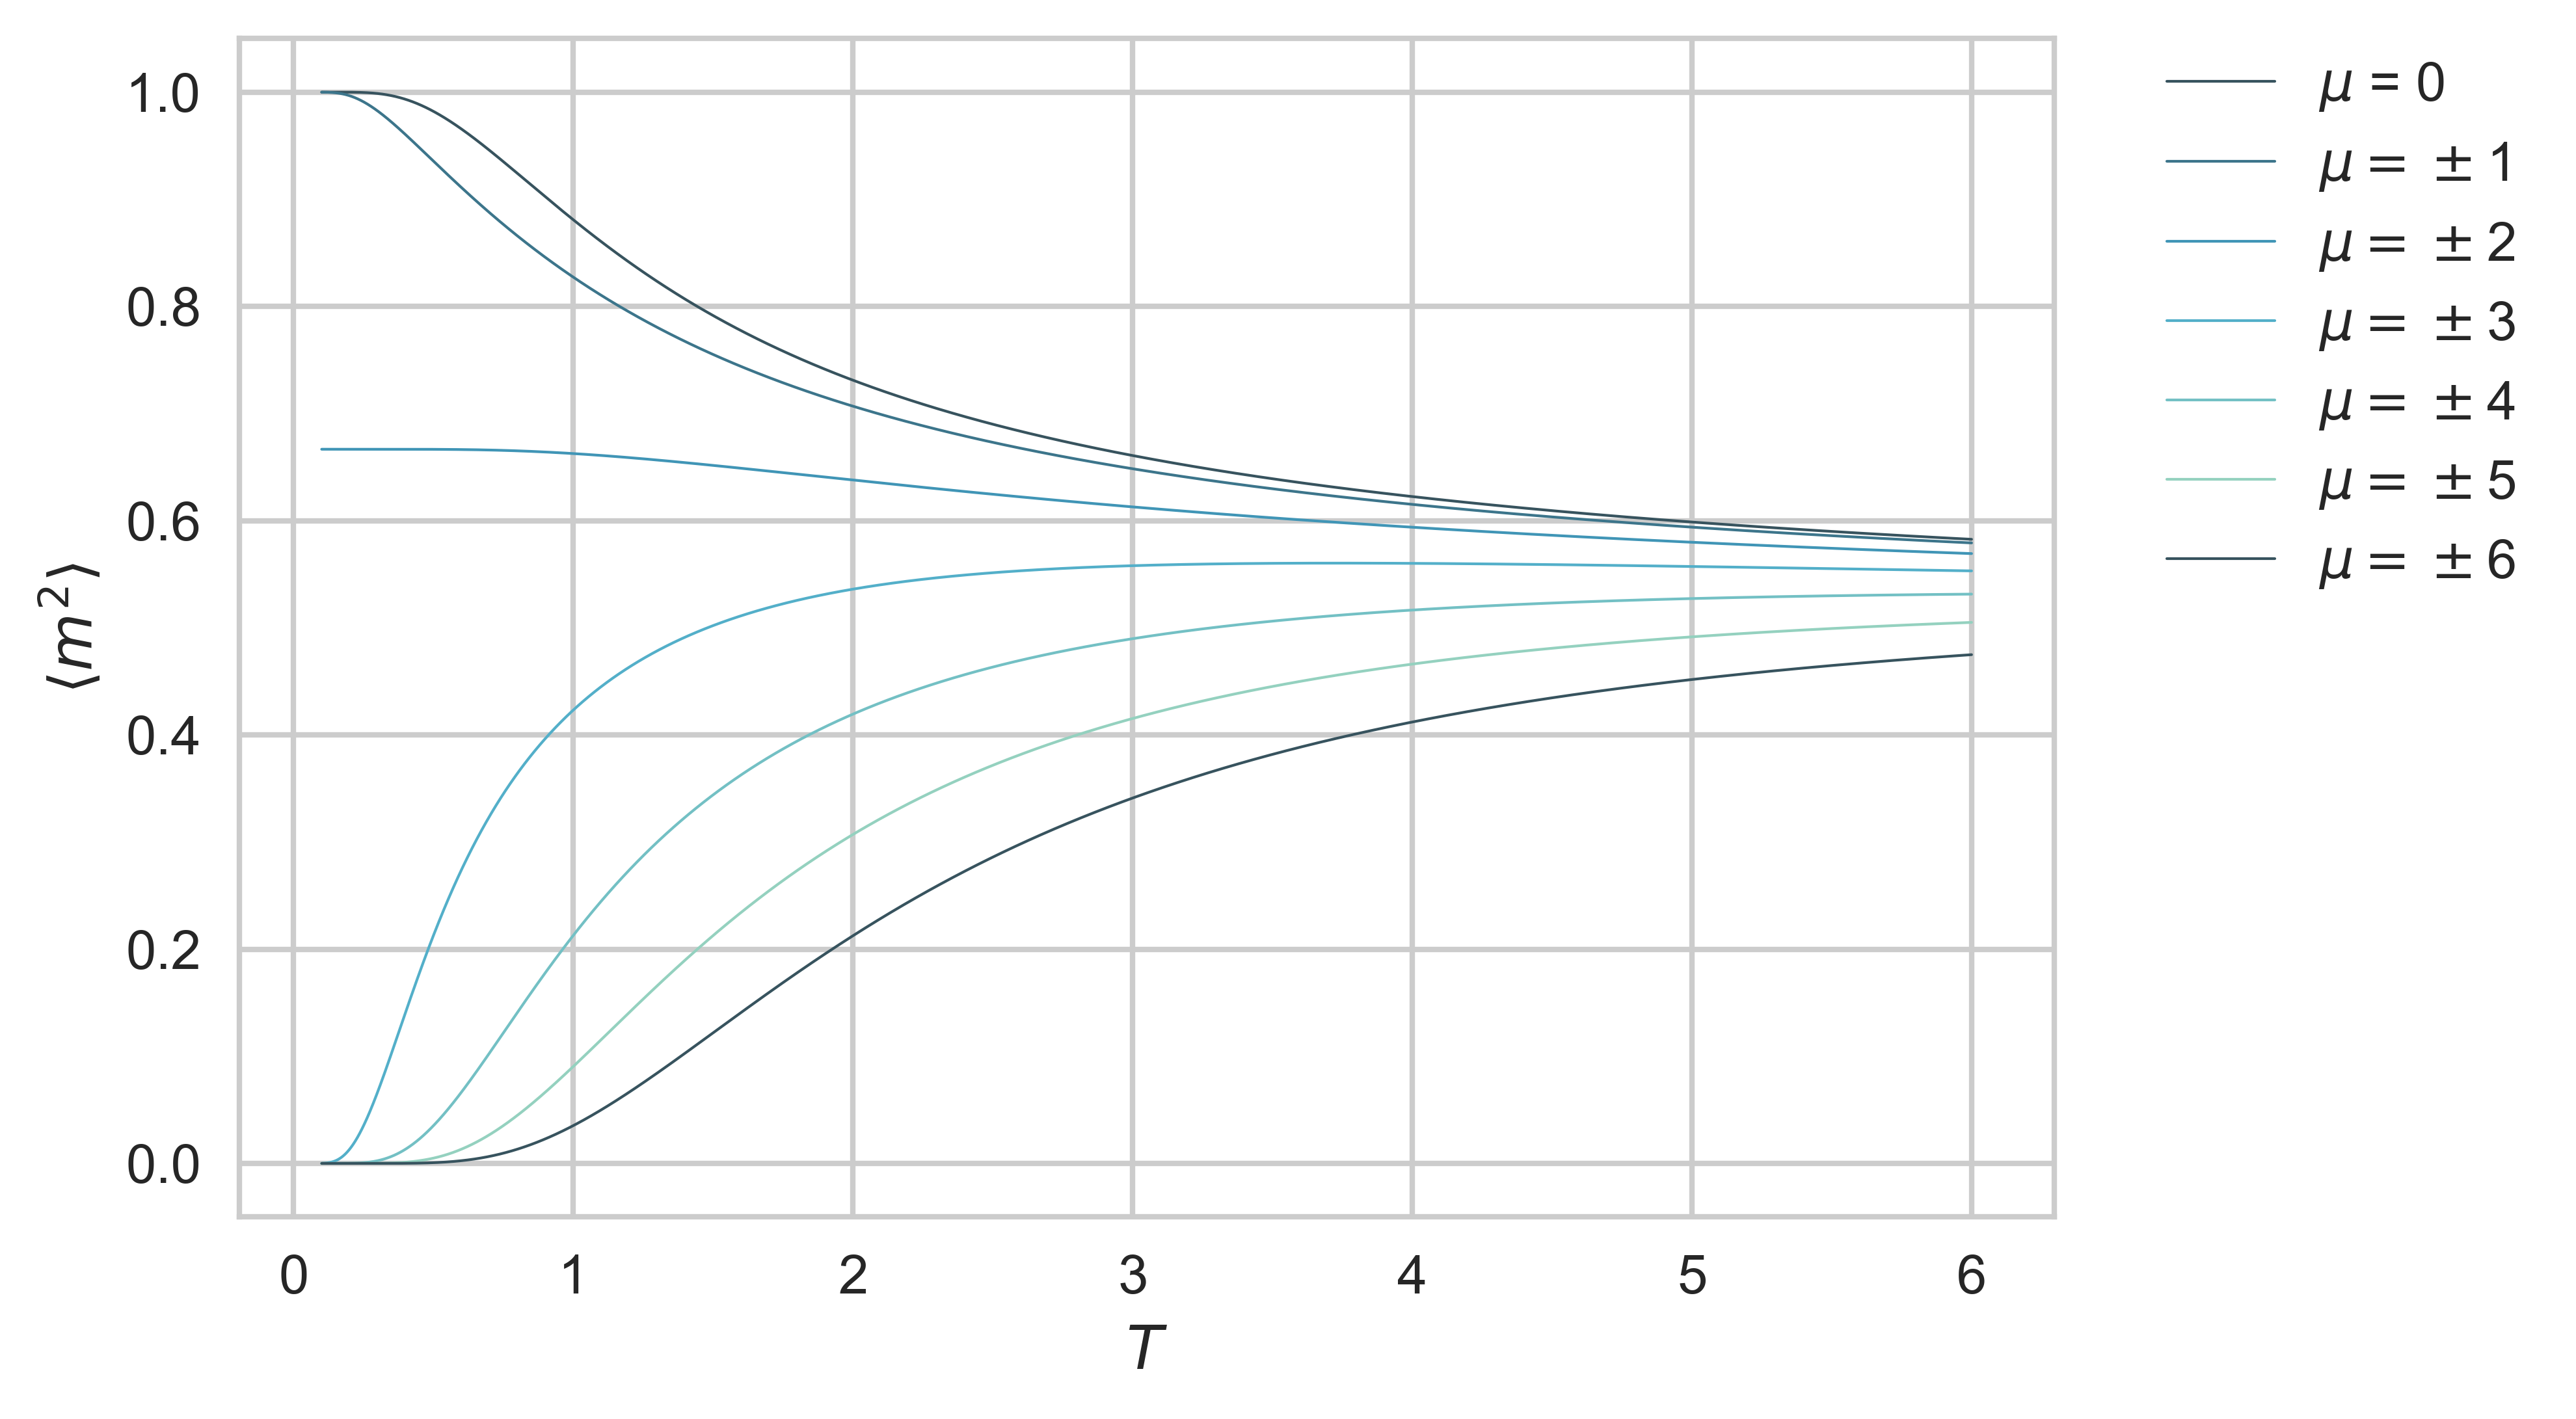
\includegraphics[width= 0.7\linewidth]{Hubbard/mSqVsT.png}
	\caption[Magnetization as a function of temperature $\left\langle m^2 \right\rangle (T)$ in the single site Hubbard model for varying chemical potential $\mu$.]{Magnetization as a function of temperature $\left\langle m^2 \right\rangle (T)$ in the single site Hubbard model for varying chemical potential $\mu$.
	Local moments develop at lower temperature.
	However, as we increase the magnitude of the chemical potential, the situation is reversed.
	At low temperatures, the site is either  doubly occupied or empty, and so the magnetization goes to zero.
	Thermal fluctuations allow the occupation of the site to fluctuate, and the magnetization to become nonzero.}
	\label{fig:mSqVsT}
\end{figure}

\subsection{The non-interacting ($\frac{U}{t} = 0$) limit}

In the $\frac{U}{t} = 0$ limit, the spin sectors become independent (since the opposite spin electrons do not interact via the on-site term) and they may be considered separately.
Thus, we omit the spin indexes of the operators in the Hamiltonian:

\begin{equation}
\mathcal{H} = -t \sum_{\left\langle i, j \right\rangle} \bigg( c_i^\dagger c_j + c_j^\dagger c_i \bigg) - \mu \sum_i n_i = \bm c^\dagger \bigg( -t \bm K - \mu \bm I \bigg) \bm c ,
\end{equation}
where we casted the Hamiltonian as a bilinear form, and defined

\begin{equation}
\bm c = \bigg[ c_1 \,\, c_2 \,\, ... \,\, c_N \bigg]^T \quad \bm c^\dagger = \bigg[c_1^\dagger \,\, c_2^\dagger \,\, ... c_N^\dagger \bigg] ,
\end{equation}
and where $\bm I$ is the identity matrix.
We also defined a matrix of zeros and ones specifying the hopping geometry, $\bm K$. The elements of the hopping matrix are simply defined by the indicator function: $K_{ij} = \mathbbm{1}_{\left\langle j_i \right\rangle} (i)$, where $\left\langle j_i \right\rangle$ is the set of neighbors $j$ of site $i$.
When writing down $\bm K$, we must specify the boundary conditions.
\acp{PBC} preserve a system's translational invariance and are advantageous because they reduce finite size effects.
An example of a quantity which is measured more accurately is energy.
In the thermodynamic limit, $N \rightarrow \infty$, the measured energy differs from the actual value by a correction of order $\mathcal{O}(\frac{1}{N^2})$ with \acp{PBC}, while for \acp{OBC}, the correction is of order $\mathcal{O}(\frac{1}{N})$ \cite{hou_numerical_2009}.
Additionally, \acp{PBC} have the property of giving site independent observables.
For example, the electron density per site does not vary with the distance to the edges of the lattice with \acp{PBC}, but it does when we use \acp{OBC}.

For concreteness, let us consider a rectangular two-dimensional lattice with $N_x \times N_y$ sites. Then, we have $\dim(\bm K) = N_x N_y \times N_x N_y $, and

\begin{equation}
\bm K = \bm I_y \otimes \bm K_x + \bm I_x \otimes \bm K_y ,
\end{equation}
where $\bm I_{x, y}$ are identity matrices of dimension $N_{x, y} \times N_{x, y}$, respectively, and $\bm K_{x, y}$ are the hopping matrices in the $x$ and $y$-directions.
For lattices in \acs{1D} or \acs{2D}, it is possible to find an exact eigendecomposition

\begin{equation}
\bm K = \bm F^T \bm \Lambda \bm F \quad \text{with}  \quad \bm F^T \bm F = \bm I ,
\end{equation}
where $\bm \Lambda = \text{diag}(\lambda_{\bm k})$ is a diagonal matrix of eigenvalues of $\bm K$.
The Hamiltonian is diagonalized:

\begin{equation}\label{eq:quadraticH}
\mathcal{H} =\tilde{\bm c}^\dagger \big( -t \bm K - \mu \bm I \big) \tilde{\bm c} = \sum_{\bm k} \varepsilon_{\bm k} \tilde{n}_{\bm k} ,
\end{equation}
where $\tilde{\bm c} = \bm F \bm c$ and $\tilde{\bm c}^\dagger = (\bm F \bm c)^\dagger$, and

\begin{equation}
\varepsilon_{\bm k} = -t \lambda_{\bm k} - \mu \quad \tilde{n}_{\bm k} = \tilde{c}_{\bm k}^\dagger \tilde{c}_{\bm k}
\end{equation}

This is equivalent to performing a canonical transformation on the annihilation (creation) operators, that preserves not their Poisson brackets, as in classical mechanics, but their anti-commutators.
Finding the eigendecomposition is equivalent to changing to Fourier space:

\begin{equation}
\tilde{c}_{\bm k}^\dagger = \frac{1}{\sqrt{N}} \sum_{} e^{i \bm k \cdot \bm R_j} c_j^\dagger ,
\end{equation}
a transformation which indeed preserves the anti-commutation relations, and the total number operator, i.e., $n = \sum_j n_j = \tilde{n} = \sum_{\bm k} n_{\bm k}$.
The $\tilde{c}_{\bm k}$-operators are equally valid electron creation/annihilation operators, obeying the same anticommutation relations as the original operators $c_i$, and the total number operator is unchanged under our transformation.
However, while the original operators create/annihilate particles at specific (spatial) sites, the new ones create/annihilate particles with momentum ${\bm k}$.
Both sets of operators describe the same physics.
Why can't this procedure be applied to the interacting case?
Well, for instance, the interaction term in the Hubbard model takes on a fairly complex form in momentum space so it is not possible to apply a similar transformation to diagonalize it.

Now, it turns out that it is easy to evaluate the partition function for quadratic Hamiltonians. If $\mathcal{H} = \bm c^\dagger \bm H \bm c$, where $\bm H$ is a $N \times N$ Hermitian matrix, then we have that

\begin{equation}\label{eq:trace_quadratic}
\text{Tr} \big[ e^{-\beta \mathcal{H} } \big] = \prod_{i=1}^N ( 1 + e^{-\beta \lambda_i } ) ,
\end{equation}
where $\lambda_i$ are the eigenvalues of $\bm H$. We present a proof of this result in appendix \ref{ap:hubbardObSol}.
It suggests that if we are able to devise some approximation to transform the quartic term of the interacting Hubbard model in a quadratic form, then we can solve it.
While this idea is essentially correct, the procedure is not straightforward.
Actually, we explore this in the next chapter to derive the simulation method that is at the basis of this work.

To complete the solution of the non-interacting case we apply the result of equation (\ref{eq:trace_quadratic}) to compute the partition function corresponding to the quadratic Hamiltonian defined in equation (\ref{eq:quadraticH}):

\begin{equation}
Z = \prod_{\bm k} ( 1 + e^{-\beta (\varepsilon_{\bm k} - \mu )} ) ,
\end{equation}
where $\varepsilon_{\bm k}$ is just the dispersion relation for a tight binding model, a standard result.
A related quantity is the density of states, counting the number of states with a given energy. For a single spin species:

\begin{equation}
N ( E ) = \frac{1}{N} \sum_{\bm k} \delta_{E,\varepsilon_{\bm k}} \rightarrow \frac{1}{(2\pi)^d} \int d\bm k \, \delta ( E - \varepsilon_{\bm k})\,\, \text{when}\,\, N\rightarrow \infty.
\end{equation}

In \acs{1D}, we have $\varepsilon_{k} = - 2 t \cos k$, which gives $N(E) = ( \pi \sqrt{ 4 t^2 - E^2 } )^{-1}$ (see appendix \ref{ap:hubbardObSol}).

Now that we have found a closed form solution for $Z$, it is again possible to find closed form expressions for observables of interest as well, namely:

\begin{enumerate}
\item the density, or average occupation of each site, $\rho$.

\begin{equation}
\rho = \left\langle n \right\rangle = \left\langle \tilde{n} \right\rangle = \frac{1}{N} \sum_{{\bm k}} \left\langle \tilde{n}_{\bm k} \right\rangle  = \frac{1}{N} \sum_{\bm k}  \frac{1}{1 + e^{\beta (\varepsilon_{\bm k} - \mu)}} = \frac{1}{N} \sum_{\bm k}  f_{\bm k} ,
\end{equation}
where $f_{\bm k} = \big(1 + e^{\beta(\varepsilon_{\bm k} - \mu)} \big)^{-1}$ is the Fermi-Dirac distribution (at half filling: $\mu = 0$).

\item the energy $E = \left\langle \mathcal{H} \right\rangle$.
\begin{equation}
E = \frac{1}{N} \sum_{\bm k} \frac{\varepsilon_{\bm k} - \mu}{1 + e^{\beta(\varepsilon_{\bm k} - \mu)}} = \sum_{\bm k} (\varepsilon_{\bm k} - \mu) f_{\bm k}
\end{equation}

\item the equal-time Green's function, which plays a key role in computing other quantities, such as correlation functions.

\begin{equation}\label{eq:eqGreenNonInt}
G_{\bm l \bm j} = \left\langle c_{\bm l} c_{\bm j}^\dagger \right\rangle = \frac{1}{N} \sum_{\bm k} e^{ i {\bm k} \cdot ( \bm l -\bm  j ) } ( 1 - f_{\bm k} )
\end{equation}

Note that the Green's function, like the Hamiltonian, is translationally invariant: $G_{\bm l \bm j} = G_{\bm l-\bm j}$. 
If we use PBCs, no site is singled out, they are all equivalent and this behavior of the Green's function should become apparent in our simulations.
\end{enumerate}

The properties of a fermionic system are dominated by particles near the Fermi surface.
On the square lattice, a unique feature called perfect nesting appears. 
For example, in \acs{2D}, the wavevector $\bm k = (\pi , \pi)$ connects symmetric regions of the Fermi surface.
This suggests that this wavevector could have a crucial role in the description of the model in the square lattice.
Indeed, as we will see, a large magnetic structure factor at $\bm k = (\pi , \pi)$ signals antiferromagnetic order.
This is a feature of the Hubbard model at half filling down to $U = 0$.
A similar effect happens in \acs{1D}, at $k = \pi$.

\begin{figure}[H]
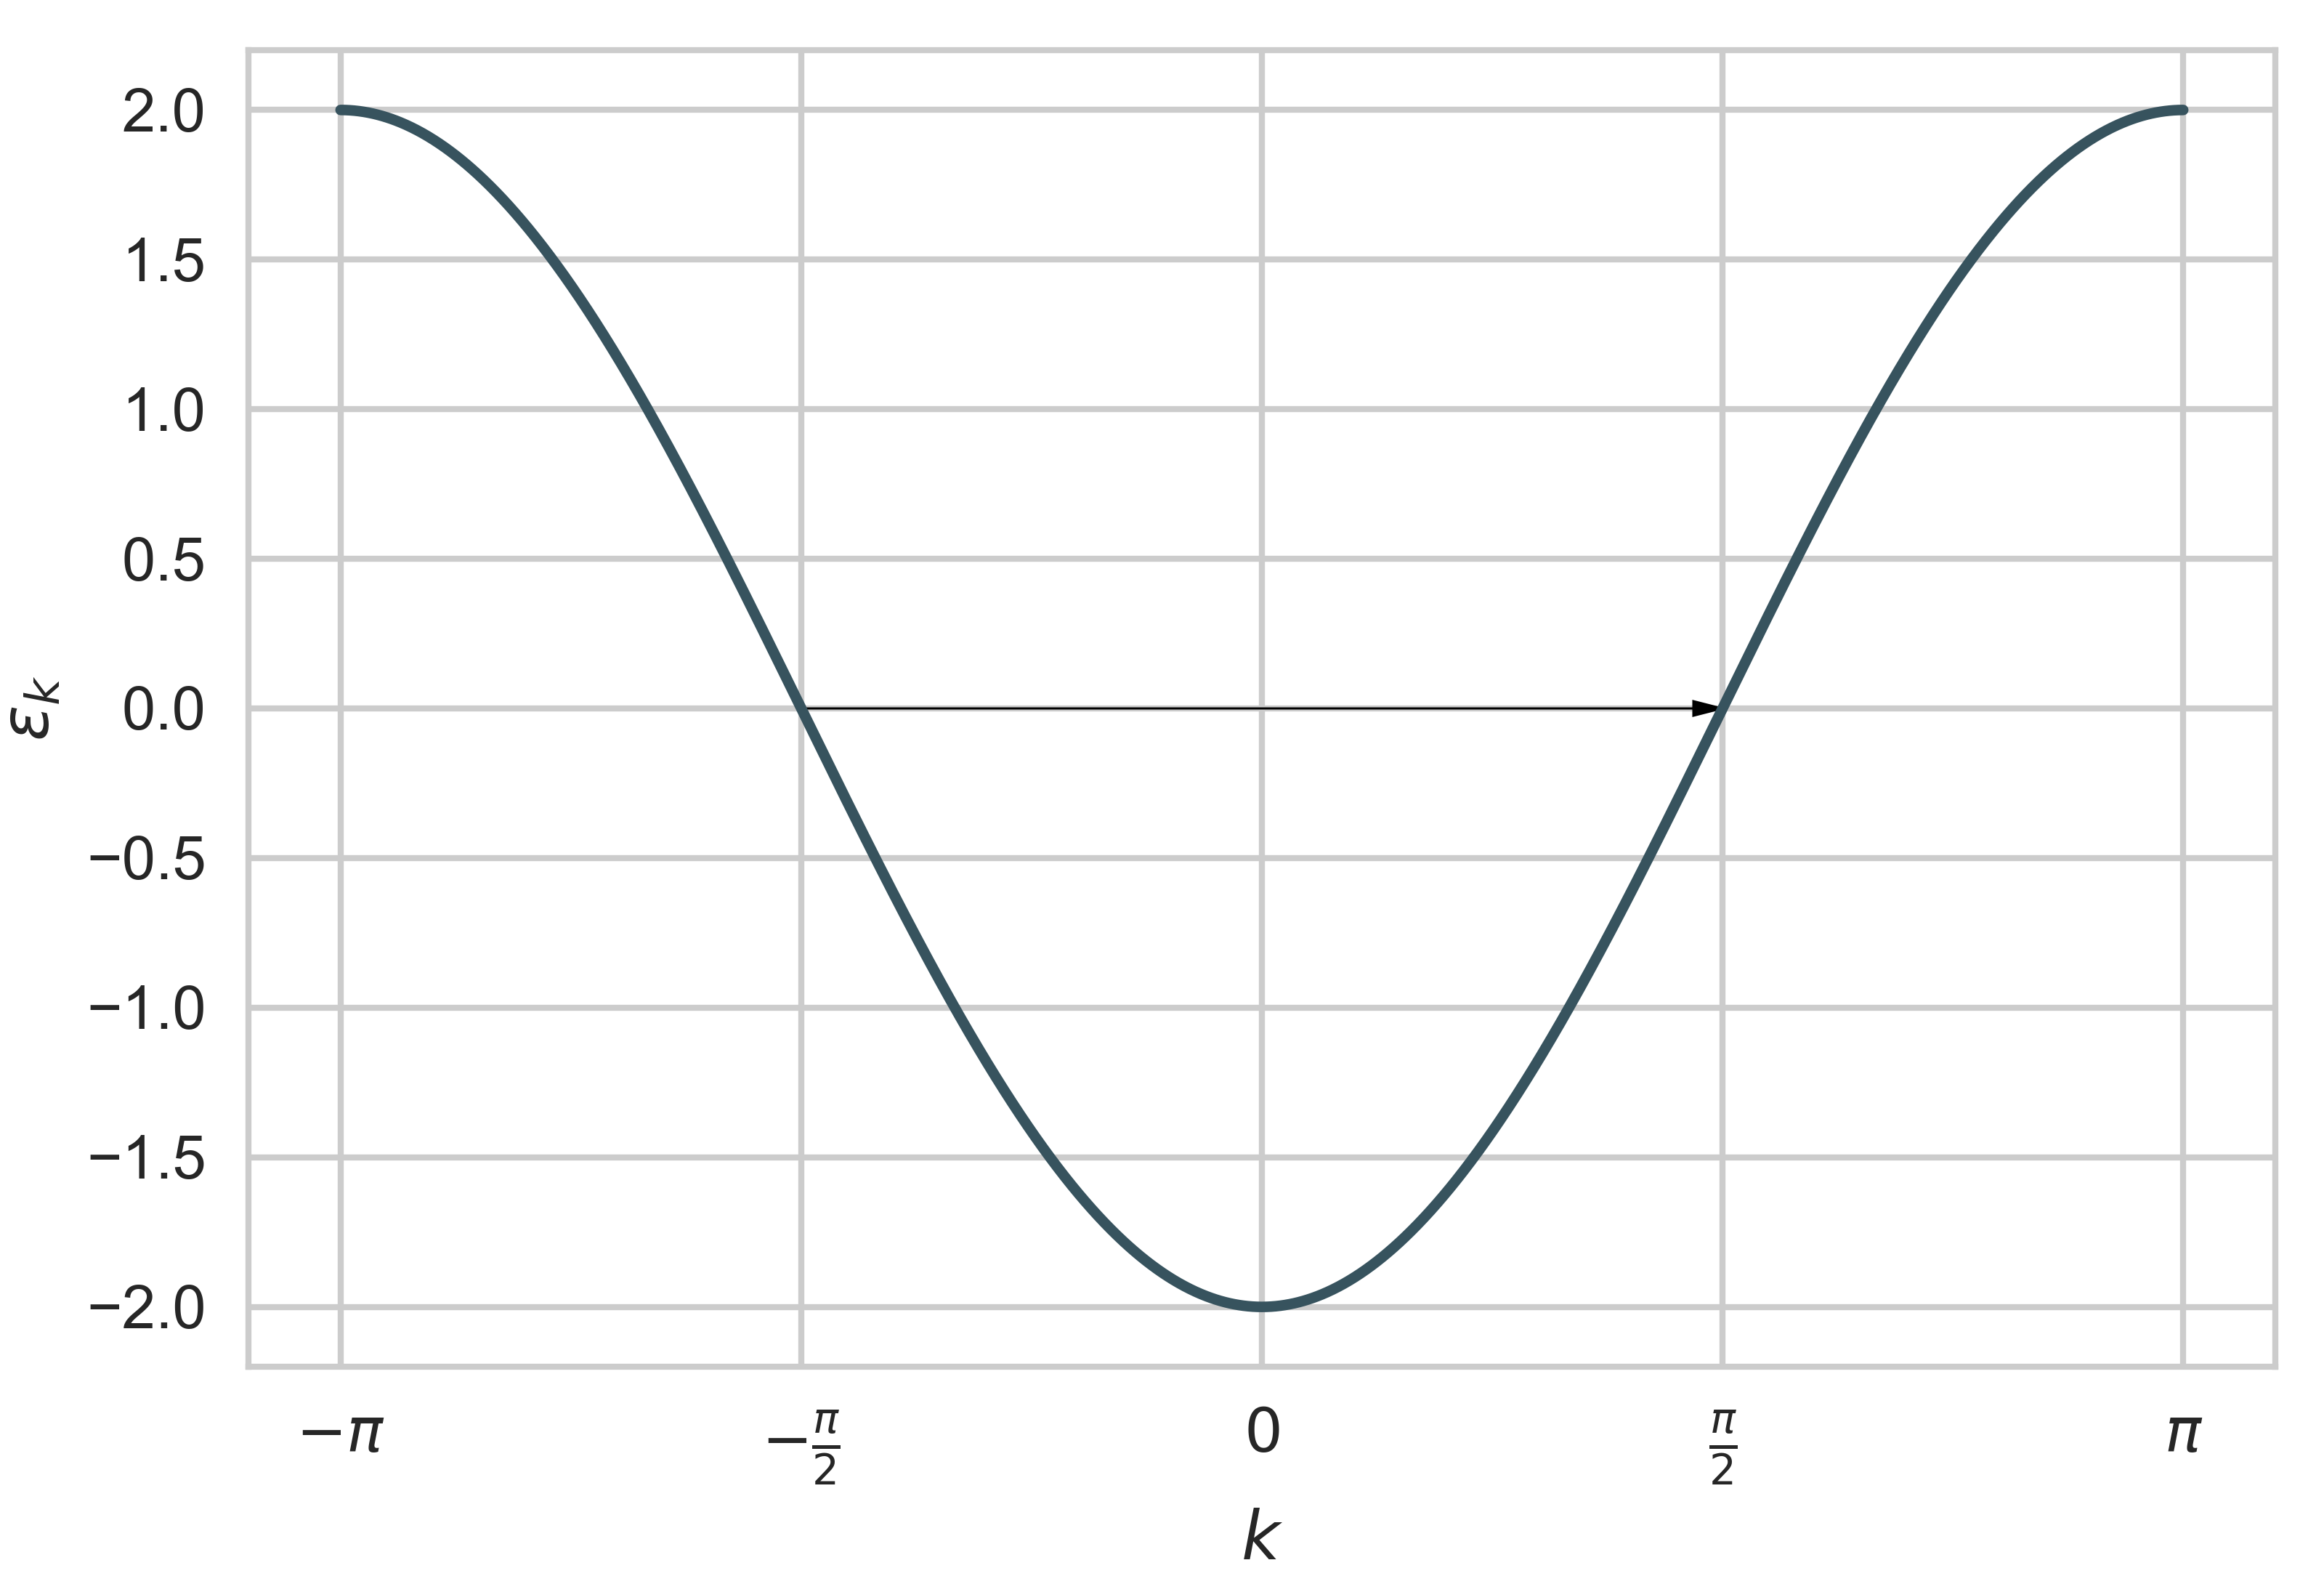
\includegraphics[width=0.55\linewidth]{Hubbard/fermiEnergy1D.png}
\hspace{-9mm}
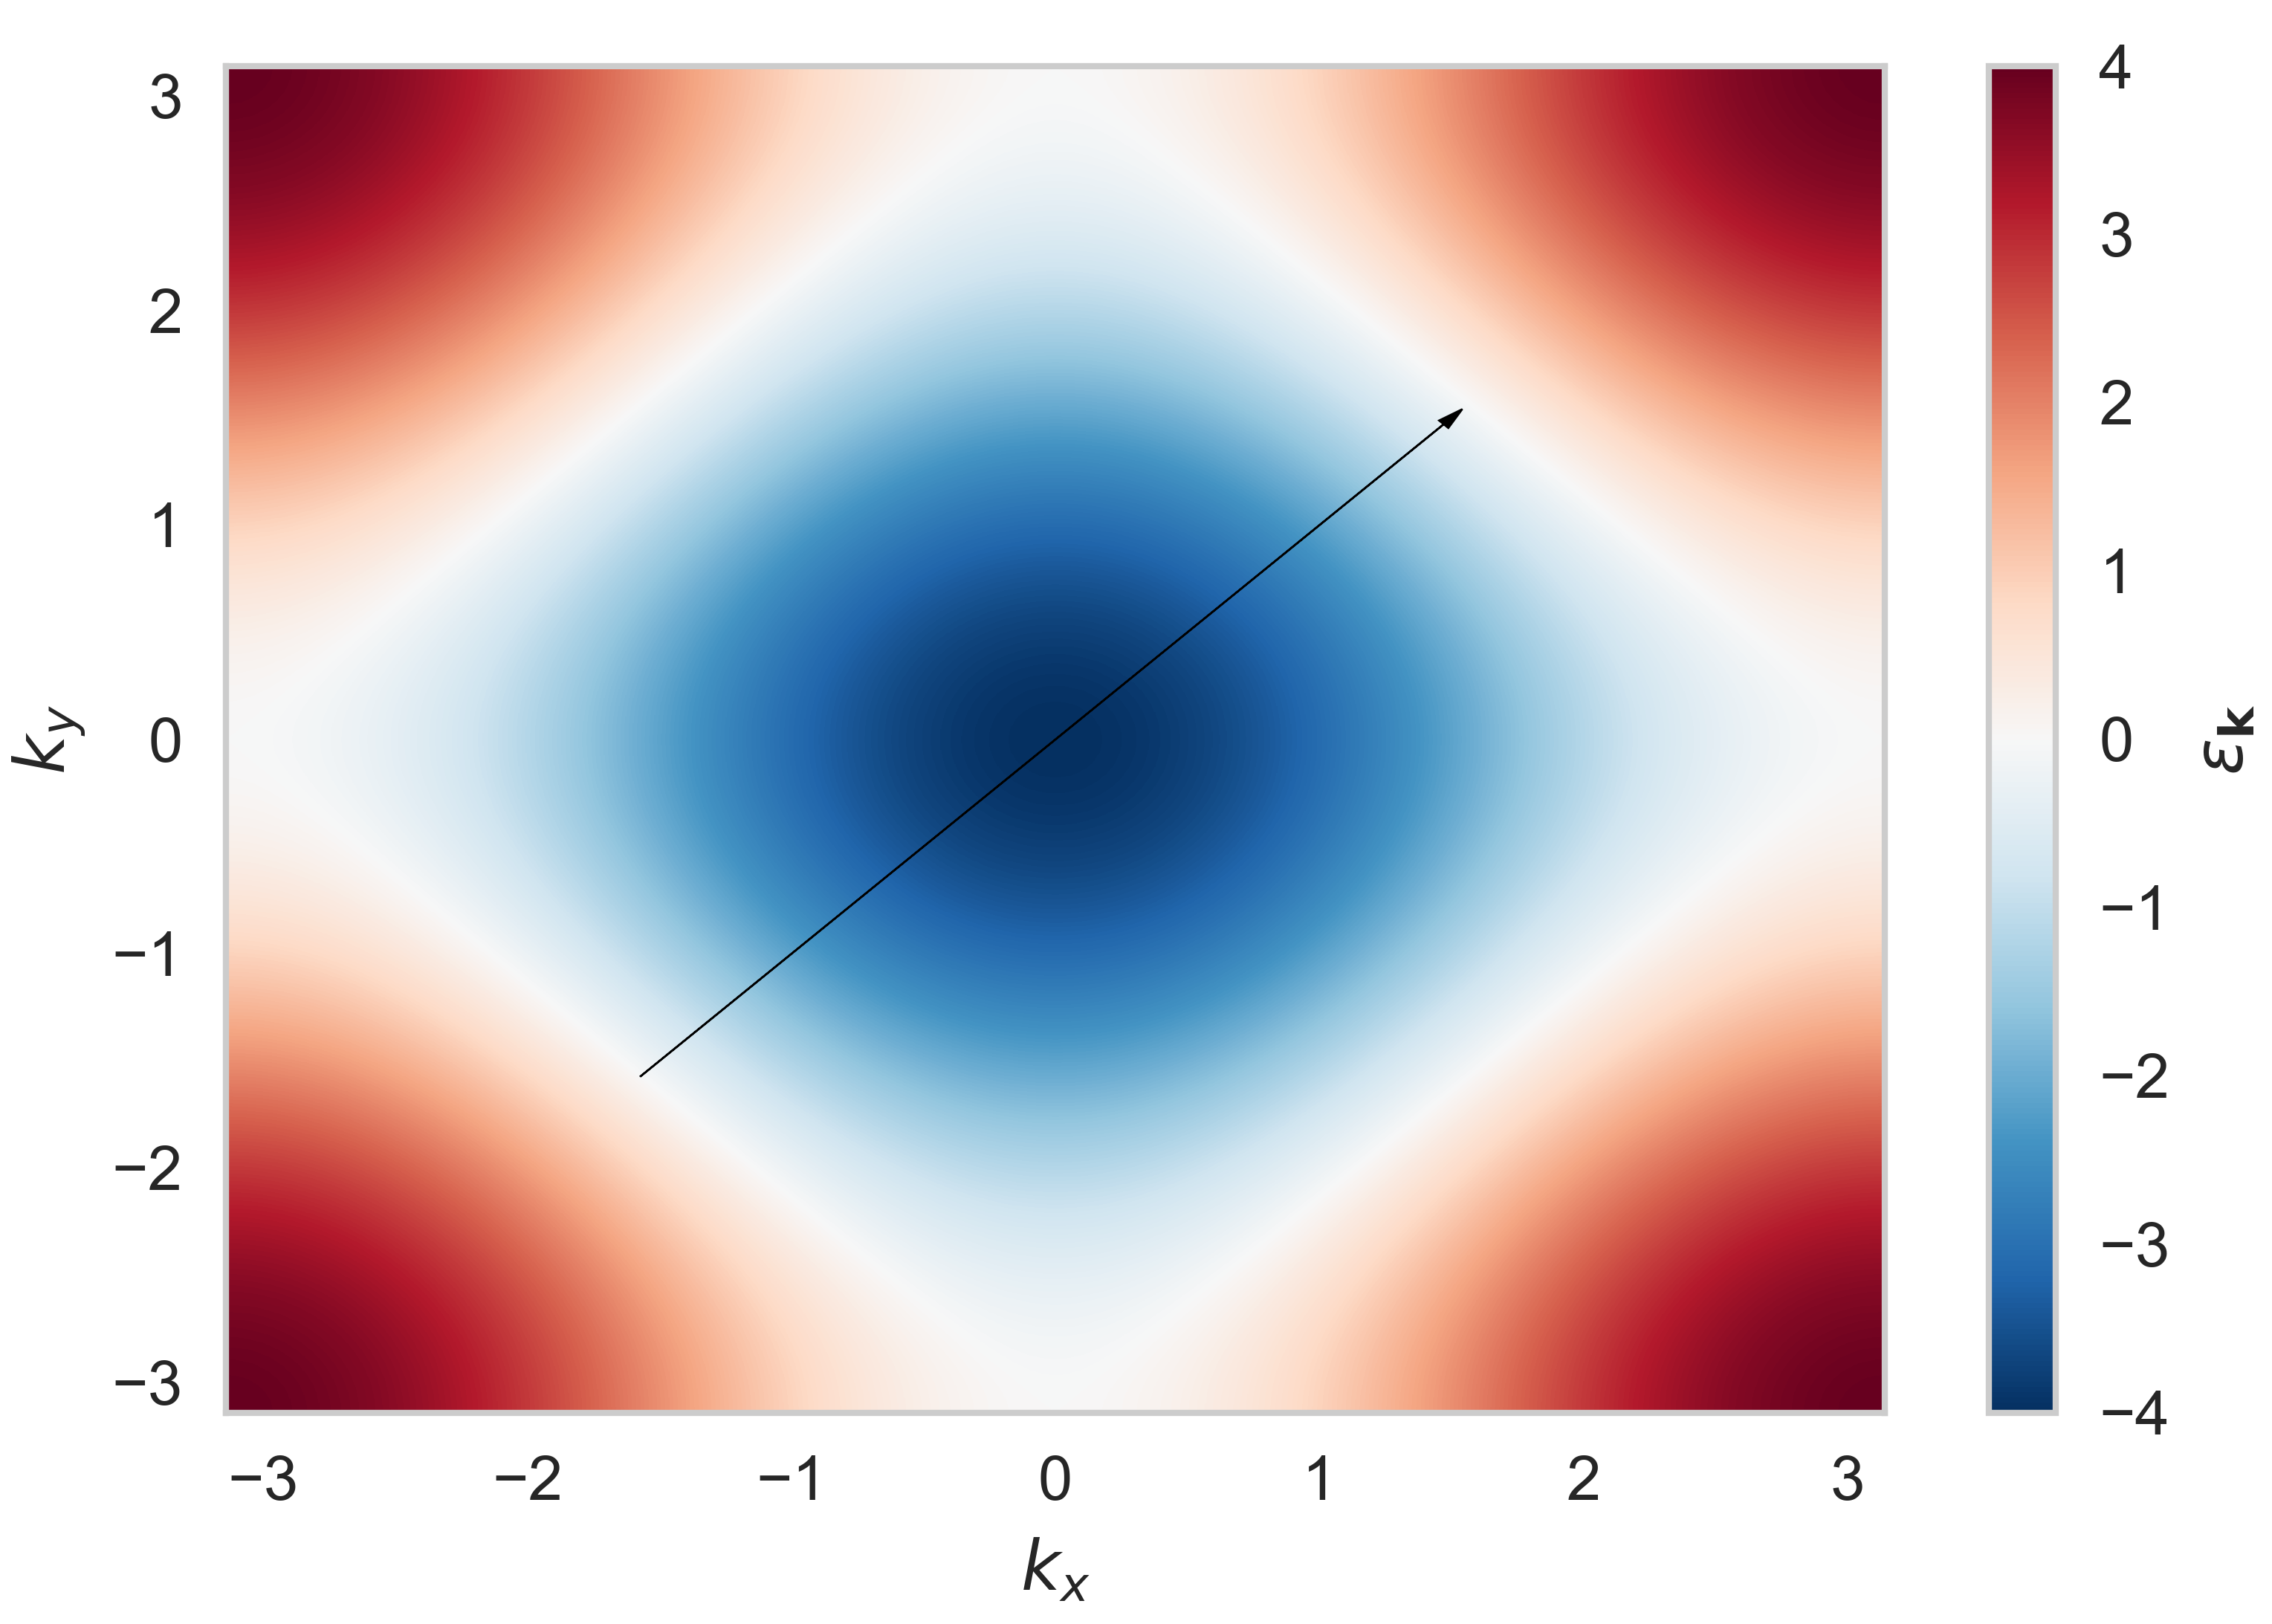
\includegraphics[width=0.49\linewidth]{Hubbard/fermiEnergy2D.png}
	\caption[Dispersion relations for the \acs{1D} chain and the square lattice in the non-interacting case.]{Dispersion relations for the \acs{1D} chain and the square lattice in the non-interacting case.
	For the square lattice, the surfaces separating the different colors are Fermi surfaces for different fillings of the lattice. In particular, for half filling ($\rho = 1, \mu = 0$), we obtain the rotated square in the white region.}
	\label{fig:fermi1D}
\end{figure}

From our analysis, we draw an important conclusion: that solving the single-particle problem, that is, obtaining $\varepsilon_{\bm k}$, gives us all the information we need about all particle sectors (any number of particles, which is controlled via the chemical potential).
When the on-site interaction is \say{turned off}, the fermions simply occupy the one-particle states according to Pauli's exclusion principle.
The single-particle sector allows us to extrapolate to obtain the behavior of a system for any number of particles simply because $U = 0$; even if the hoppings were not uniform, this would hold.
The hoppings need not even be only between nearest neighbors, and in general we could even consider a chemical potential varying from site to site.
All we require is that the Hamiltonian is a quadratic form of the fermion operators.
